\section{Fixing Dead Salmons with Hypothesis Testing}
\label{app:exp}

Consider an interpretability method $M$ that aims to explain a neural network $f$ for some input behavior $P_{\bU}$, we note $\mathfrak{C}$ the tuple $(f, P_{\bU})$ as done in the main paper. The method produces an explanation $\hat{e}$ from finite observations from $\mathfrak{C}$, possibly under interventions. This tentative explanation could take the form of a circuit, a set of important features, concept activation vectors, or any other hypothesis class. We might wonder how to prevent dead salmon artifacts from arising with the interpretability method $M$? 

A simple, direct, and natural solution is to frame this question as a hypothesis test against a null hypothesis where the observed explanation arises from random computation. Already, for probing, \citet{ravichander-etal-2021-probing} discusses the possibility of comparing the probe against a probe trained on random embeddings. The general idea is to construct a family of null models represented by a distribution $P_{\tilde{\mathfrak{C}}}$, which preserves the network’s architectural properties while disrupting the specific computational mechanisms we aim to explain. Such null models can be obtained, for example, via full weight randomization, random orthogonal transformations of representations, or label shuffling (recovering the standard permutation test).  

For a given interpretability method, we define a test statistic $T(\hat{e}, \mathfrak{C})$ that quantifies explanatory fit for the interpretability task at hand. For example, for probing methods, $T$ could be test accuracy; for circuit discovery, $T$ could measure behavioral fidelity; for attribution methods, $T$ could quantify the correlation between attribution scores and actual intervention effects.

Applying the intepretability method $M$ to one null model $\tilde{\mathfrak{C}}^{(b)}$ from the randomized family yields explanations $\tilde{e}^{(b)} = M(\tilde{\mathfrak{C}}^{(b)})$ and corresponding null statistics $T_{\text{null}}^{(b)} = T(\tilde{e}^{(b)}, \tilde{\mathfrak{C}}^{(b)})$. Then, following standard procedure, the Monte Carlo estimated $p$-value is:
\begin{equation}
\hat{p} = \frac{1 + \sum_{b=1}^B \mathbb{I}\{T_{\text{null}}^{(b)} \ge T_{\text{obs}}\}}{B + 1},
\end{equation}
where $T_{\text{obs}} = T(\hat{e}, \mathfrak{C})$. The addition of 1 to both the numerator and denominator ensures Type~I error control:
$
\Pr(\hat{p} \le \alpha \mid H_0) \le \alpha,
$ where $H_0$ is the null hypothesis~\citep{north2002note,phipson2010permutation}. By design, when the randomization includes full weight reinitialization, no dead salmon artifacts can remain.


\subsection{Experiments}
To illustrate the hypothesis test, we experiment with three probing tasks.

\textbf{Sentiment Analysis (IMDb).}
We reuse the IMDB sentiment classification setup from Figure~\ref{fig:illus}. For each layer of \texttt{BERT-base-uncased}, we extract the average sentence embedding and train a linear probe to predict binary sentiment. We also train probes on $k{=}20$ random reinitializations of the model, and evaluate statistical significance using the hypothesis test described above. All probes are trained and evaluated on 1000 sentences with 10-fold cross-validation.
Figure~\ref{fig:experiments}(A) reports (i) the average probe accuracy at each layer for the pretrained model, the randomized models, and a random guessing baseline, and (ii) the corresponding effect sizes relative to random guessing and to randomized models. While all pretrained layers outperform random guessing with large effect sizes, none are statistically distinguishable from the random reinitializations under the new test. Later layers, however, show a clear upward trend in effect size relative to randomized models.

\textbf{Syntactic Structure (POS Tagging).}
We next assess token-level syntactic information using POS-tagging probes~\citep{tenney-etal-2019-bert}. For each layer of \texttt{BERT-base-uncased}, we extract contextual token embeddings and train logistic regression probes on a subset of CoNLL-2003, one probe per layer that should work for all tokens and all POS tags. As above, we also train probes on $k{=}20$ random reinitializations and apply the same statistical test. Probes are evaluated with 10-fold cross-validation on 500 sentences.
Figure~\ref{fig:experiments}(B) reports the layer-wise probe accuracy and effect sizes relative to a majority baseline and to randomized models. Consistent with prior work, POS accuracy peaks in middle layers~\citep{tenney-etal-2019-bert}. However, when tested against randomized models rather than random guessing, only the middle layers remain statistically above chance, and the effect sizes are substantially reduced. This shows that testing against random computations eliminates many positive findings while still allowing for genuine positive discoveries where structure is robust.

\begin{figure}
    \centering
    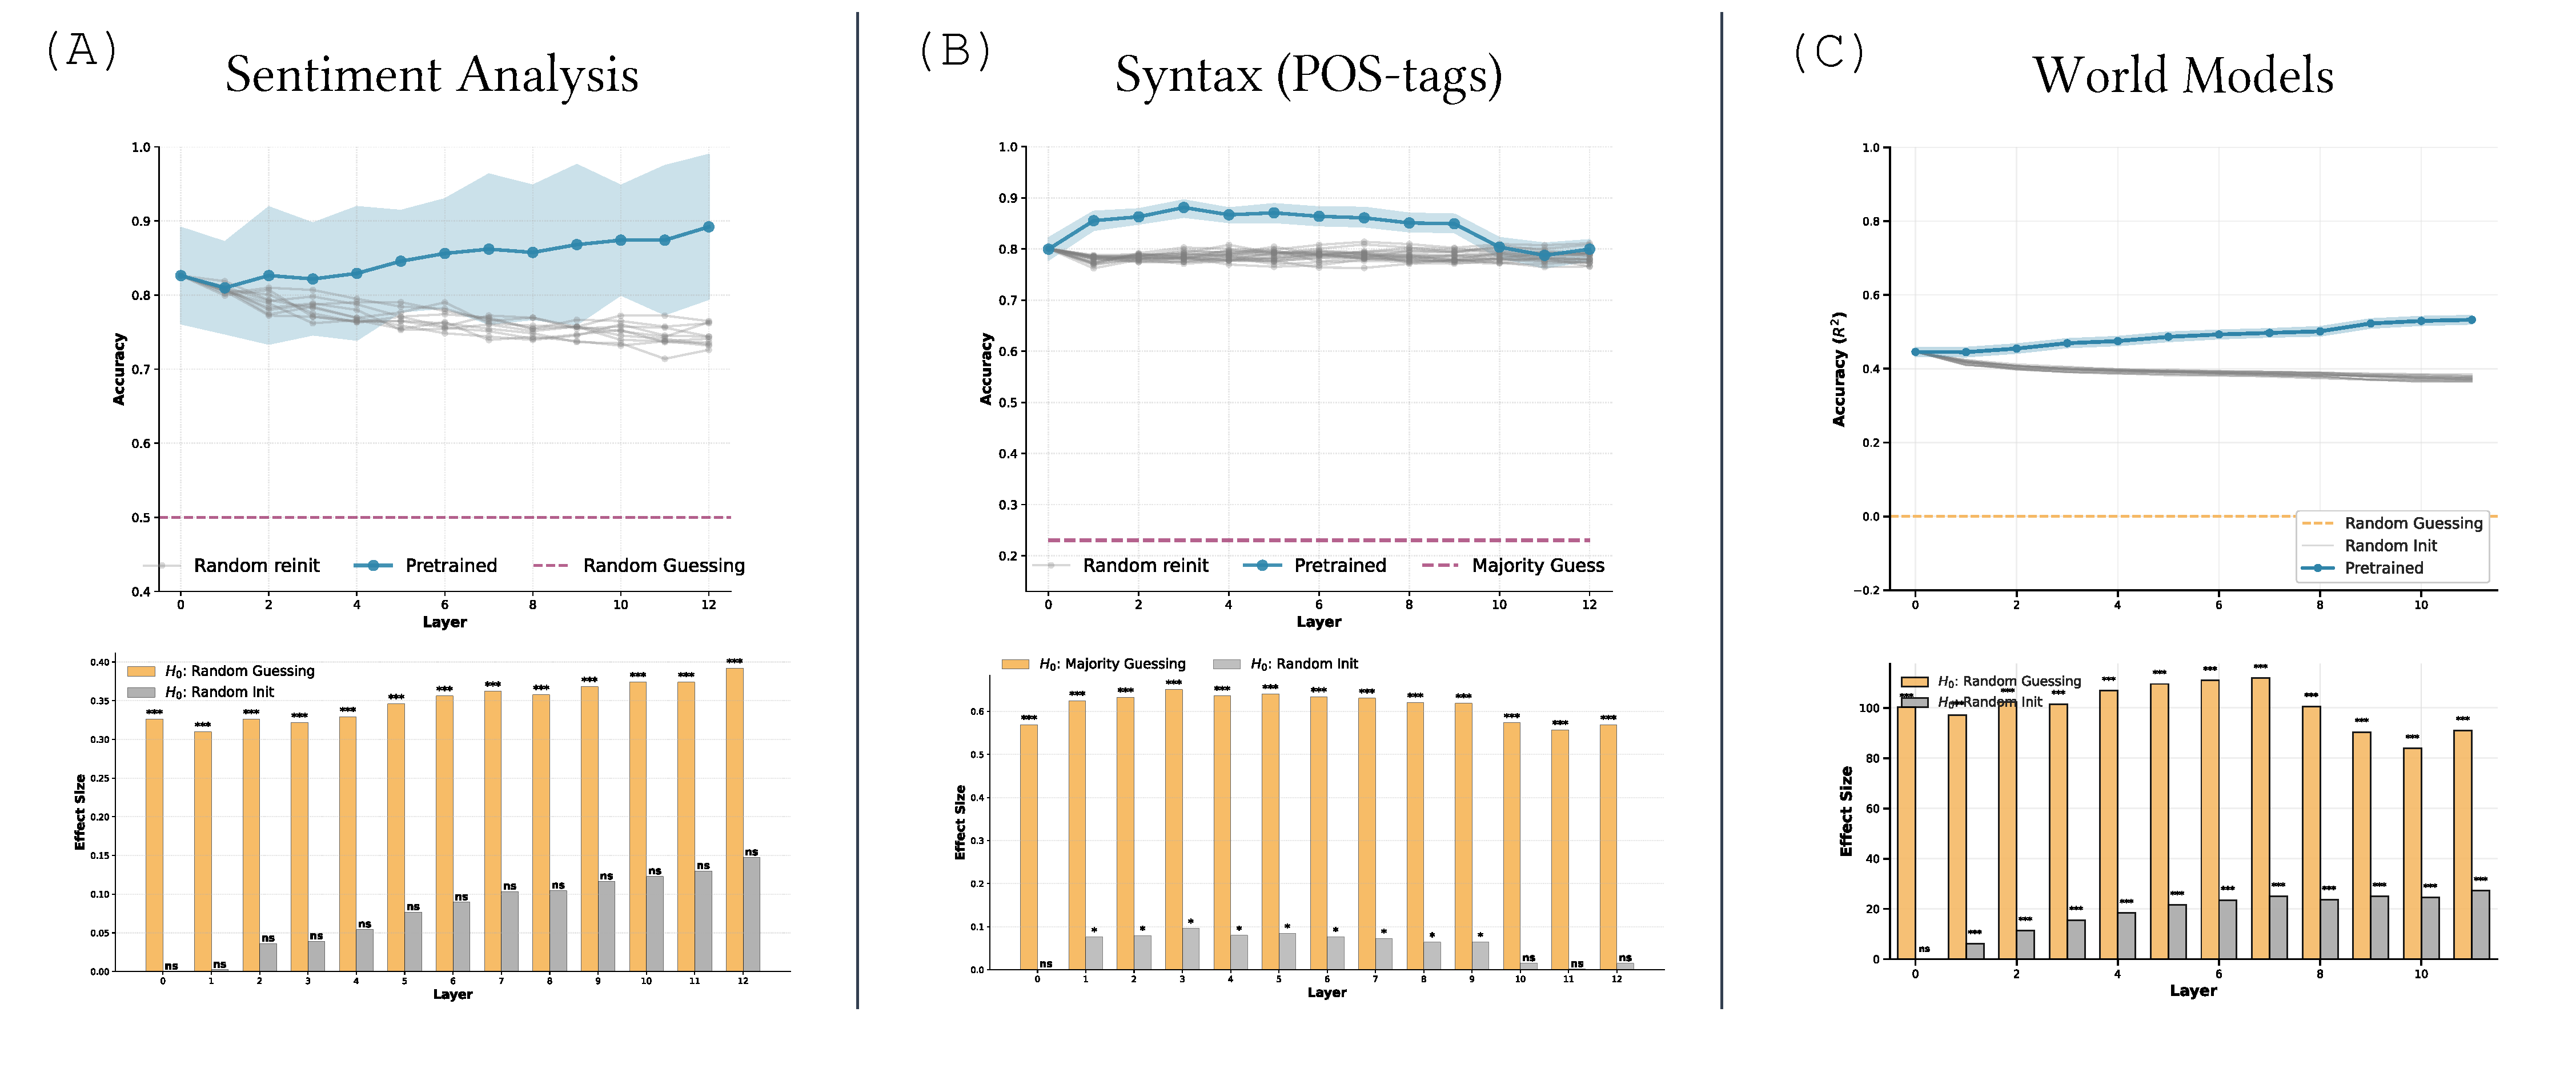
\includegraphics[width=0.9\linewidth]{images/expe.pdf}
    % \includegraphics[width=0.3\linewidth]{images/expe_wm_pythia.pdf}
    \caption{(A) Sentiment analysis experiment where probes on pretrained BERT are compared against probes trained on random computation. (B) Same experiment based on predicting syntactic labels (POS tags). (C) Reproducing the first experiment of Table 2 in \cite{gurnee2024language}, probing for indications of world models on pythia-160m.}
    \label{fig:experiments}
\end{figure}

\textbf{World Models (Space and Time).}
Finally, we investigate the emergence of linear representations of space using the ``world places'' dataset from~\citep{gurnee2024language}. Using \texttt{pythia-160m}, we extract average residual stream activations on each token of place names and train linear ridge regression probes to predict their geospatial coordinates (latitude and longitude). We compare the pretrained model against $k=20$ baselines where transformer block weights are randomized while embeddings remain fixed. Probes are evaluated using $R^2$ scores with 10-fold cross-validation.
Figure~\ref{fig:experiments}(C) reveals that raw embeddings (Layer 0) contain latent spatial structure ($R^2 \approx 0.12$), significantly outperforming random guessing ($Z \approx 100$). Passing these embeddings through randomized transformer blocks decreases linear readout ($R^2 \approx 0.38$). In contrast, the pretrained model's layers slightly improve this spatial linearity relative to the random baseline, suggesting that deeper layers progressively construct a more coherent spatial representation. By the final layers, the learned structure statistically surpasses the random baseline ($Z \approx 25$), confirming that the model eventually learns to encode space explicitly beyond the geometry inherent in the embeddings.



% \section{Interpretability Methods as Statistical Inference Problems}

\begin{table}[ht]
\centering
\renewcommand{\arraystretch}{1.25}
\begin{tabular}{@{}p{3.2cm}p{5.1cm}p{5.1cm}@{}}
\toprule
\textbf{Method} & \textbf{Hypothesis space $\mathcal{E}$ (surrogate model)} & \textbf{Typical causal query $q(\mathfrak{C})$ and error criterion $D$} \\
\midrule
\textbf{Performance benchmarking} 
& Single scalar summarizing predictive performance (e.g., accuracy, calibration, perplexity).  
& \textit{Observational query:} output score distribution under $P_{\bU}$.  
Error: difference in expected performance metrics, e.g., $|{\mathbb E}[f(\bU)] - {\mathbb E}[\hat{f}(\bU)]|$. \\ 
\midrule
\textbf{Probing (linear / diagnostic classifiers)} 
& Linear or shallow classifiers mapping internal activations to target variables (e.g., part-of-speech tags).  
& \textit{Observational query:} conditional distribution $P(Y\,|\,\text{activations})$.  
Error: classification loss. \\ 
\midrule
\textbf{Feature attributions (saliency, SHAP, Integrated Gradients)} 
& Input-level additive surrogates assigning contribution scores so that $f(x)$ is approximated by $\sum_i e_i(x)\,x_i$ relative to a baseline.  
& \textit{Counterfactual queries:} local (additive) approximation of model behavior around inputs $x$.  
Error: fidelity loss between model predictions and surrogate reconstruction \\ 
\midrule
\textbf{Concept-based methods (e.g., TCAV, ACE, concept bottleneck models)} 
& Surrogates mapping internal activations to interpretable concept variables and modeling $f$’s dependence on them.  
& \textit{Interventional queries:} model sensitivity or dependence on interpretable concept activations within latent space.  
Error: deviation between surrogate-predicted and model-predicted sensitivities (e.g., directional derivative mismatch). \\ 
\midrule
\textbf{Circuit discovery} 
& Subgraphs of the computational graph representing causal mechanisms.  
& \textit{Interventional queries:}  outputs distribution under targeted ablations encoded by the circuit.  
Error: consistency in output distribution, e.g.,
$KL\big(P_{\mathfrak{C}}(Y \mid U) \, \| \, P_{\text{circuit}}(Y \mid U)\big)$ \\ 
\midrule
\textbf{Causal tracing (patching, mediation analysis)} 
& Scalar importance scores over units or connections inferred from intervention or mediation effects.  
& \textit{Counterfactual mediation queries:} total, direct, or indirect effect of node $V_i$ on target $Y$.  
Error: difference between predicted and empirical effects. \\ 
\midrule
\textbf{Causal abstraction / model-level alignment} 
& High-level structural causal model with mappings from low-level network variables $\bV$ to abstract variables $\bZ$.  
& \textit{Interventional invariance queries:} the actions of abstracting from $V$ to $Z$ and intervening should commute.
Error: causal abstraction error, measuring causal alignment as violation of commutative properties of abstraction and intervention. \\ 
\bottomrule
\end{tabular}
\caption{Interpretability methods as instances of the statistical--causal framework of \emph{surrogate models}. Each method specifies a hypothesis class $\mathcal{E}$, causal query family $q(\mathfrak{C})$, and associated error measure $D$ quantifying how faithfully the surrogate answers the queries.}
\label{tab:interpretability_methods}
\end{table}